% Báo cáo Đề tài 05 — Chinese–Vietnamese sentence alignment (dạng bài báo, 8–10 trang)
% Biên dịch: tectonic bao_cao.tex   (hoặc xelatex; KHÔNG dùng pdflatex vì fontspec/xeCJK)
\documentclass[12pt,a4paper]{article}

% ---------- font & ngôn ngữ
\usepackage{fontspec}
\setmainfont{Times New Roman}
\setmonofont{Courier New}[Scale=0.88]
\usepackage{xeCJK}
\setCJKmainfont{Songti SC}
\usepackage[vietnamese]{babel}

% ---------- bố cục
\usepackage[margin=2.3cm]{geometry}
\usepackage{parskip}
\usepackage{booktabs,array,multirow}
\usepackage{graphicx}
\usepackage{amsmath,amssymb}
\usepackage{xcolor}
\usepackage{listings}
\usepackage{tikz}
\usetikzlibrary{arrows.meta,positioning}
\usepackage[hidelinks]{hyperref}
\emergencystretch=3em
\usepackage{caption}
\usepackage{url}
\captionsetup{font=small,labelfont=bf}
\usepackage{titlesec}
\titlespacing*{\section}{0pt}{1.2em}{0.4em}
\titlespacing*{\subsection}{0pt}{0.9em}{0.3em}

\lstset{basicstyle=\ttfamily\footnotesize,breaklines=true,frame=single,
        backgroundcolor=\color{gray!8},columns=fullflexible,keepspaces=true}
\newcommand{\code}[1]{\texttt{#1}}
\newcommand{\B}[1]{\textbf{#1}}
\newcommand{\croco}{CroCoAlign}

% ---------- thông tin (sửa cho đúng)
\newcommand{\truong}{TRƯỜNG ĐẠI HỌC \ldots}
\newcommand{\khoa}{KHOA \ldots}
\newcommand{\monhoc}{Xử lý ngôn ngữ tự nhiên}
\newcommand{\hocvien}{Ngô Trường Minh Đạt}
\newcommand{\gvhd}{\ldots}
\newif\ifcover \covertrue     % \coverfalse để bỏ trang bìa

\begin{document}

% =====================================================================
\ifcover
\begin{titlepage}
\centering
{\large \truong\\ \khoa\par}
\vspace{3cm}
{\Large \B{BÁO CÁO CUỐI KỲ}\\[0.3cm] Môn: \monhoc\par}
\vspace{2cm}
{\LARGE \B{Đề tài 05}\\[0.4cm]
 \B{Dóng hàng câu Hán -- Việt cho \emph{Đại Việt Sử Ký Toàn Thư}}\\[0.4cm]
 \large bằng mô hình \croco{} (EACL 2024): tái lập, đánh giá trên gold gán tay\\ và cải tiến bằng giải mã đơn điệu\par}
\vfill
\begin{tabular}{rl}
Học viên: & \hocvien\\
Giảng viên hướng dẫn: & \gvhd\\
\end{tabular}
\vspace{1.5cm}

{\large Tháng 9 năm 2026}
\end{titlepage}
\setcounter{page}{1}
\fi

% =====================================================================
\begin{center}
{\Large\B{Dóng hàng câu Hán -- Việt cho \emph{Đại Việt Sử Ký Toàn Thư} bằng \croco{}:\\[2pt]
tái lập, đánh giá trên gold gán tay và cải tiến}}\\[8pt]
{\large \hocvien}\\[2pt]
{\small Môn \monhoc{} -- Đề tài 05 -- Mã nguồn, dữ liệu và kết quả: kho \code{CK\_XLNNTN}, nhánh \code{eval-manual-gold}}
\end{center}

\begin{center}\B{Tóm tắt}\end{center}
\begingroup\small
Dóng hàng câu (\emph{sentence alignment}) là bước tạo ngữ liệu song song cho dịch máy và nghiên cứu văn bản cổ. Báo cáo
này thực hiện đề tài 05: xây dựng ngữ liệu Hán cổ -- Việt hiện đại từ bản fulltext \emph{Đại Việt Sử Ký Toàn Thư}
(14 mục Ngoại kỷ, 1\,703 câu Hán / 1\,833 câu Việt), cài đặt và chạy lại \croco{} \cite{crocoalign} -- hệ dóng hàng
neural có ngữ cảnh, đạt SOTA trên Opus Books -- từ mã nguồn gốc với checkpoint chính thức trên stack phần mềm hiện đại,
rồi đánh giá và cải tiến. Khác với cách đánh giá bằng \emph{silver gold} sinh từ chính mô hình (vòng tròn), chúng tôi gán
tay 185 nhóm liên kết trên 3 mục làm tập kiểm tra độc lập, tách DEV/TEST, chọn cấu hình bằng cross-validation, và so với
hai baseline phi-neural. Kết quả: \croco{} zero-shot đạt $F_1$ strict 0,529 (tinh chỉnh: 0,565); giữ nguyên bộ mã hoá
LaBSE của checkpoint nhưng thay bộ giải mã bằng quy hoạch động đơn điệu đạt \B{0,918} (+39 điểm); một baseline thuần từ
vựng Hán-Việt không cần mô hình neural đạt \B{0,934}. Phân tích cho thấy với song ngữ dịch sát, ràng buộc thứ tự quan trọng
hơn chất lượng embedding, và silver gold không thể dùng để chấm mô hình cùng gốc. Toàn bộ pipeline tái lập bằng một lệnh
trên CPU.
\endgroup

% =====================================================================
\section{Giới thiệu}

Cho hai tài liệu là bản dịch của nhau, \emph{dóng hàng câu} tìm các nhóm câu tương ứng ($1$-$1$, $1$-$n$, $n$-$1$,
$n$-$m$, hoặc câu không có cặp). Đây là bước nền cho dịch máy, tra cứu song ngữ và số hoá văn bản cổ. Cặp Hán cổ --
Việt của \emph{Đại Việt Sử Ký Toàn Thư} (ĐVSKTT) có ba đặc thù: (i) văn bản Hán cổ \B{không có dấu câu}, nên ngay việc
xác định ``câu'' đã là bài toán; (ii) khoảng cách ngôn ngữ và thời đại lớn -- mô hình đa ngữ hiện đại được huấn luyện trên
tiếng Trung hiện đại, không phải văn ngôn thế kỷ XV; (iii) bản dịch chèn nhiều chú giải, niên đại và tách/gộp câu, nên
dóng hàng không thuần $1$-$1$.

Đề tài yêu cầu: (1) tiền xử lý dữ liệu cho phù hợp mô hình; (2) cài đặt và chạy lại \croco{} \cite{crocoalign} theo bài
báo EACL 2024; (3) thực nghiệm, đánh giá, và có thể cải tiến. Đóng góp của báo cáo:
\begin{itemize}
  \item Pipeline cào và tiền xử lý 14 mục ĐVSKTT, giải quyết tách câu Hán cổ bằng dấu câu của \emph{phiên âm Hán-Việt}
  đi kèm ở nguồn (Mục~\ref{sec:data}).
  \item Tái lập \croco{} với checkpoint chính thức trên torch~2.x / transformers~5.x mà không sửa mã gốc (Mục~\ref{sec:setup}).
  \item Bộ gold \B{gán tay} 185 nhóm, giao thức DEV/TEST + cross-validation, scorer độc lập khớp \code{evaluate.py}
  gốc, hai baseline phi-neural (Mục~\ref{sec:eval}).
  \item Hai cải tiến giữ nguyên bộ mã hoá của \croco{} nhưng thay bộ giải mã bằng quy hoạch động đơn điệu, tăng
  $F_1$ strict từ 0,529 lên 0,918; và bằng chứng định lượng rằng silver gold sinh từ mô hình thiên vị cấu trúc
  (Mục~\ref{sec:results}--\ref{sec:analysis}).
\end{itemize}

% =====================================================================
\section{Nghiên cứu liên quan}

\B{Phương pháp thống kê.} Gale và Church \cite{galechurch} dóng hàng bằng tỉ lệ độ dài câu và quy hoạch động (DP)
đơn điệu với các bước $1$-$1$, $1$-$0$, $0$-$1$, $1$-$2$, $2$-$1$, $2$-$2$; đơn giản nhưng vẫn là baseline mạnh khi hai
bản đi song song. Hunalign và Bleualign \cite{bleualign} thêm từ điển hoặc bản dịch máy làm tín hiệu.
\B{Phương pháp nhúng câu.} Vecalign \cite{vecalign} dùng embedding đa ngữ (LASER) với DP xấp xỉ đa mức, tuyến tính theo
độ dài, và định nghĩa thước đo strict/lax $P/R/F_1$ mà \croco{} và báo cáo này dùng lại. LaBSE \cite{labse} là bộ nhúng
câu 109 ngôn ngữ huấn luyện bằng translation-ranking, cho cosine giữa bản dịch cao và ổn định, được dùng làm bộ mã hoá
trong \croco{}.
\B{\croco{}} \cite{crocoalign} là hệ đầu tiên end-to-end, có ngữ cảnh: quyết định từng cặp câu bằng một bộ phân loại
neural trên embedding đã được ngữ-cảnh-hoá, không cần DP; đạt macro-$F_1$ strict 87,5 trên 20 cặp ngôn ngữ Opus Books
so với 85,9 của Vecalign. Điểm khác biệt của báo cáo này là dữ liệu \emph{ngoài phân phối} (Hán cổ, gần đơn điệu tuyệt
đối) và việc kiểm chứng \croco{} bằng gold gán tay thay vì gold tự sinh.

% =====================================================================
\section{Mô hình \croco{}}\label{sec:model}

\subsection{Kiến trúc}
Hình~\ref{fig:arch} tóm tắt kiến trúc (theo \cite{crocoalign}, kiểm chứng lại trong mã nguồn
\code{pl\_modules/pl\_module.py}). Cho câu nguồn $s_1..s_n$ và câu đích $t_1..t_m$:
\begin{enumerate}
  \item \B{Bộ nhúng câu} LaBSE (\emph{đóng băng}) cho $E_{s_i}, E_{t_j}\in\mathbb{R}^{768}$.
  \item \B{Bộ mã hoá ngữ cảnh}: một Transformer kiểu DistilBERT khởi tạo ngẫu nhiên (6 lớp, 6 đầu, dropout 0,2), nhận
  \emph{chuỗi embedding câu} của một tài liệu làm đầu vào (\code{inputs\_embeds}) và nhờ positional embedding + attention
  tạo ra embedding có ngữ cảnh $C_{s_i}, C_{t_j}$. Đây là đóng góp chính của bài báo: câu được đặt trong ngữ cảnh các câu
  lân cận trước khi so khớp.
  \item \B{Đầu phân loại}: với mọi cặp $(i,j)$ tính tích Hadamard $C_{s_i}\odot C_{t_j}$, đưa qua
  $\text{Linear}(768{\to}384)\to\text{Dropout}\to\text{ReLU}\to\text{Linear}(384{\to}1)$ và sigmoid, cho xác suất
  $M_{ij}$; ngưỡng 0,5 quyết định liên kết. Mỗi câu nguồn có thể nối với 0, 1 hoặc nhiều câu đích và ngược lại.
\end{enumerate}

\begin{figure}[t]\centering
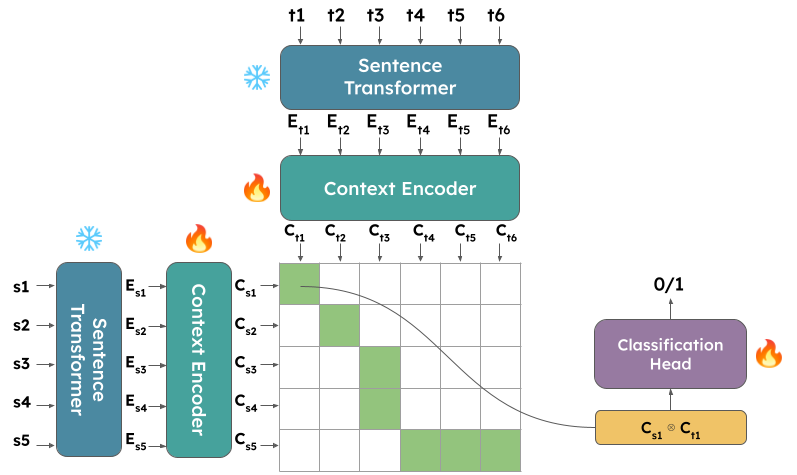
\includegraphics[width=0.82\linewidth]{fig_crocoalign_arch.png}
\caption{Kiến trúc \croco{} (hình của tác giả \cite{crocoalign}, kho GitHub Babelscape/CroCoAlign): bộ nhúng câu đóng
băng, bộ mã hoá ngữ cảnh và đầu phân loại được huấn luyện; ma trận $n\times m$ với ô xanh là cặp dóng hàng.}
\label{fig:arch}
\end{figure}

\subsection{Huấn luyện}
Hàm mất mát là binary cross-entropy trên toàn ma trận, với $\hat M$ là ma trận gold:
\[\mathcal{L}=-\frac{1}{nm}\sum_{i,j}\Big[\hat M_{ij}\log\sigma(M_{ij})+(1-\hat M_{ij})\log\big(1-\sigma(M_{ij})\big)\Big].\] Dữ liệu: Opus Books (16 ngôn ngữ, 64 cặp, 251 sách; 231 sách huấn luyện, 10 kiểm định,
10 kiểm tra); 77\% liên kết là $1$-$1$. Cấu hình (\code{conf/nn/default.yaml}): AdamW, lr $5\cdot10^{-6}$ (bài báo:
$10^{-5}$), weight decay 0,01, warmup 10\%, batch 64 câu, gradient clipping 10, early stopping (patience 10) theo
$F_1$ strict trên tập kiểm định; huấn luyện trên RTX 3090~Ti. Checkpoint công bố (2,31~GB) chứa cả LaBSE lẫn bộ mã hoá
ngữ cảnh và đầu phân loại; báo cáo này \B{không huấn luyện lại} mà dùng checkpoint đó (zero-shot với Hán cổ -- Việt).

\subsection{Suy luận trên tài liệu dài}\label{sec:inference}
Vì không đưa cả tài liệu vào GPU, \croco{} suy luận theo lô (\code{batch\_size}=32 câu):
\B{Pointing} -- với mỗi lô nguồn, dùng FAISS tìm $k$ câu đích có cosine LaBSE cao nhất với câu đầu lô, \B{loại ứng viên
có vị trí tương đối lệch quá} \code{min\_dist}=0,05, thử từng cửa sổ đích quanh ứng viên và giữ cửa sổ cho nhiều liên
kết nhất; \B{Recovery} -- nếu một câu nguồn bị nối với các câu đích không kề nhau, chọn lại bằng cosine LaBSE của câu
(\code{labse}) hoặc của câu kèm $N{=}3$ câu lân cận (\code{labse-batch}, biến thể tốt nhất trong bài báo). Điểm quan
trọng cho phân tích sau này: \B{mỗi cặp được quyết định độc lập}, không có ràng buộc thứ tự toàn cục như DP.

% =====================================================================
\section{Dữ liệu và tiền xử lý (Yêu cầu 1)}\label{sec:data}

\subsection{Nguồn và cấu trúc}
Bản fulltext ĐVSKTT của nomfoundation.org gồm 73 mục, mỗi mục nhiều trang khắc in, phân trang phía server bằng POST
\code{curPg}. Mỗi trang có một bảng HTML: ô thứ nhất chứa \emph{chữ Hán và phiên âm Hán-Việt xen kẽ theo block}
\begin{center}\small\code{<chữ Hán> [trang*dòng*cột] <phiên âm Hán-Việt, có dấu câu>}\end{center}
ô thứ hai (``Dịch Quốc Ngữ'') là bản dịch tiếng Việt hiện đại, cùng thứ tự. Ví dụ một block:
\begin{center}\small
按黃帝時建萬國以交趾界於西南遠在百粵之表 \code{[1a*4*1]} \emph{Án: Hoàng đế thời, kiến vạn quốc, dĩ Giao Chỉ giới ư
Tây Nam, viễn tại Bách Việt chi biểu.}\\
$\rightarrow$ ``Xét: Thời Hoàng Đế dựng muôn nước, lấy địa giới Giao Chỉ về phía Tây Nam, xa ngoài đất Bách Việt.''
\end{center}

\subsection{Hai phát hiện then chốt}
\B{(1) Dấu câu của phiên âm cho phép tách câu Hán cổ.} Người biên soạn đã đặt dấu chấm/chấm hỏi ở phiên âm; mỗi block
Hán tương ứng đúng một đoạn phiên âm kết thúc bằng dấu kết câu, nên block $\approx$ câu. Không cần mô hình tách câu Hán cổ.
\B{(2) Phiên âm là tín hiệu từ vựng nối hai bản.} Bản dịch hiện đại giữ nguyên rất nhiều từ Hán-Việt (\emph{Sĩ Nhiếp,
Giao Châu, Thái thú, Kiến An, Long Biên}); độ trùng âm tiết giữa phiên âm và câu Việt đo được mà không cần mô hình.
Phát hiện này dùng cho cả gán nhãn tay (Mục~\ref{sec:gold}) lẫn baseline (Mục~\ref{sec:baselines}).

\subsection{Pipeline}
\begin{figure}[h]\centering\small
\resizebox{\linewidth}{!}{\begin{tikzpicture}[node distance=4mm and 5mm, every node/.style={font=\small},
  box/.style={draw,rounded corners=2pt,align=center,minimum height=8mm,inner sep=3pt,fill=gray!6},
  arr/.style={-{Latex[length=2mm]}}]
\node[box] (web) {nomfoundation\\HTML};
\node[box,right=of web] (raw) {\code{scrape\_dvsktt.py}\\\code{raw/*.jsonl} (theo trang)};
\node[box,right=of raw] (pp) {\code{preprocess.py}\\tách block Hán, câu Việt};
\node[box,right=of pp] (out) {\code{zh.jsonl} / \code{vi.jsonl}\\\code{blocks.tsv} (Hán$\leftrightarrow$phiên âm)};
\draw[arr] (web)--(raw); \draw[arr] (raw)--(pp); \draw[arr] (pp)--(out);
\end{tikzpicture}}
\caption{Pipeline tiền xử lý. Đầu ra \code{zh.jsonl}/\code{vi.jsonl} đúng định dạng \croco{}
(mỗi dòng \code{\{"ids":[...],"text":[...]\}}); \code{blocks.tsv} giữ phiên âm cho gán nhãn và baseline.}
\end{figure}

\code{scrape\_dvsktt.py} chạy được với \code{requests} hoặc thuần \code{urllib} (POST multipart tự dựng), có retry và
delay 0,8~s/trang. \code{preprocess.py}: tách block bằng biểu thức chính quy trên marker
\code{[\textbackslash d+[ab]*\textbackslash d+*\textbackslash d+]}, giữ ký tự CJK (kể cả vùng CJK mở rộng B/F),
tách câu Việt theo \code{. ! ? ;} sau khi bỏ nội dung trong ngoặc vuông (chú giải, niên đại). Bảng~\ref{tab:data} thống kê
14 mục đã xử lý.

\begin{table}[h]\centering\footnotesize
\caption{14 mục Ngoại kỷ sau tiền xử lý. DEV = mục 1--3, TEST = mục 7, 9, 10.}\label{tab:data}
\begin{tabular}{llrrr@{\hspace{1.2em}}llrrr}
\toprule
\B{Mục} & \B{Vai trò} & \B{Trang} & \B{Hán} & \B{Việt} & \B{Mục} & \B{Vai trò} & \B{Trang} & \B{Hán} & \B{Việt}\\
\midrule
1 Hồng Bàng thị & DEV & 9 & 80 & 90     & 8 thuộc Ngô--Tề & -- & 27 & 309 & 312\\
2 Nhà Thục & DEV & 13 & 112 & 125       & 9 Tiền Lý & TEST & 6 & 64 & 65\\
3 Nhà Triệu & DEV & 35 & 331 & 354      & 10 Triệu Việt Vương & TEST & 6 & 51 & 59\\
4 thuộc Tây Hán & -- & 2 & 22 & 24      & 11 Hậu Lý & -- & 6 & 44 & 46\\
5 Trưng Nữ Vương & -- & 2 & 19 & 22     & 12 thuộc Tuỳ--Đường & -- & 33 & 350 & 357\\
6 thuộc Đông Hán & -- & 9 & 83 & 94     & 13 Nam Bắc phân tranh & -- & 5 & 56 & 55\\
7 Sĩ Vương & TEST & 11 & 75 & 91        & 14 Nhà Ngô & -- & 14 & 107 & 139\\
\midrule
\multicolumn{10}{l}{\B{Tổng}: 190 trang, \B{1\,703} câu Hán, \B{1\,833} câu Việt}\\
\bottomrule
\end{tabular}
\end{table}

Nhiễu thực tế cần lưu ý: bản dịch có $\approx$8\% câu nhiều hơn bản Hán (chú giải, tách câu); vài câu cụt do lỗi ở
nguồn (\emph{``KỶ TRIỆU V''}, \emph{``là Ki''}); câu bị cắt ngang trang ở cả hai bản (\emph{``Thời Thứ sử Chu'' | ``Phù bị
giặc Di giết\ldots''}); chú giải dài (truyền thuyết Chử Đồng Tử: 1 block Hán ứng với 6 câu Việt).

% =====================================================================
\section{Cài đặt và chạy lại \croco{} (Yêu cầu 2)}\label{sec:setup}

Mã nguồn được đưa vào kho dưới dạng git submodule ghim commit \code{2e93992} (HEAD upstream, 09/2024). Repo ghim
\code{torch==1.11}, \code{pytorch-lightning==1.5}, \code{transformers==4.20}, \code{faiss-gpu==1.7.2} -- không cài được
trên phần cứng hiện có (GPU Blackwell sm\_120; macOS arm64). Bảng~\ref{tab:install} liệt kê các vướng mắc; nguyên tắc
là \B{không sửa mã gốc}, mọi vá lỗi nằm trong wrapper ở \code{scripts/} (\code{run\_align.py}, \code{run\_eval.py},
\code{run\_eval\_tuned.py}).

\begin{table}[h]\centering\small
\caption{Vướng mắc khi cài đặt và cách khắc phục}\label{tab:install}
\begin{tabular}{p{3.4cm}p{5.4cm}p{6.6cm}}
\toprule
\B{Vấn đề} & \B{Nguyên nhân} & \B{Khắc phục}\\
\midrule
torch ghim không chạy & RTX 5050 (sm\_120) không tương thích \code{torch==1.11}; macOS không có CUDA & torch 2.11+cu128 (WSL2) / torch 2.14 CPU (macOS)\\
\code{faiss-gpu} không cài được & chỉ có cho CUDA cũ & \code{faiss-cpu}; dữ liệu vài nghìn câu, đủ nhanh\\
Nạp checkpoint lỗi & PL~2.6 bỏ \code{\_load\_model\_state} mà \code{nn\_core.load\_model} gọi; torch~2.6 mặc định \code{weights\_only=True}; sentence-transformers~$\ge$3 đổi tên module \code{auto\_model}$\to$\code{model} & loader tự viết: giải nén \code{.ckpt.zip}, \code{torch.load(weights\_only=False)}, ánh xạ lại khoá state\_dict; kết quả \code{missing=0}, chỉ 2 buffer \code{position\_ids} thừa (vô hại)\\
Thiếu phụ thuộc nn-core & phải cài \code{--no-deps} để không bị ép lightning cũ & thêm GitPython, python-dotenv\\
Đường dẫn tương đối & \code{evaluate.py} ghi \code{results\_*.tsv} vào CWD & runner \code{cd} vào thư mục đích, dùng đường dẫn tuyệt đối\\
\bottomrule
\end{tabular}
\end{table}

\B{Kiểm chứng.} (i) Ví dụ EN$\leftrightarrow$IT kèm repo cho kết quả đúng, kể cả câu tiêu đề không có cặp; (ii) chạy
end-to-end Hán$\leftrightarrow$Việt với checkpoint chính thức trên hai môi trường: WSL2 + RTX 5050 (env
\code{crocoalign}: Python 3.10, torch 2.11+cu128, PL 2.6.5) và macOS arm64 CPU (\code{.venv}: Python 3.10, torch 2.14,
transformers 5.16, sentence-transformers 6.0, PL 2.6.5, faiss-cpu, nn-template-core 0.1.1). Số liệu trong báo cáo lấy từ
lần chạy macOS; toàn bộ phần cần torch (\croco{} gốc + tuned trên TEST, cải tiến trên 14 mục $\times$ 64 cấu hình) chạy
hết trong $\approx$15 phút CPU, mỗi lượt \croco{} trên 190 câu TEST $\approx$5 phút kể cả nạp mô hình.

% =====================================================================
\section{Phương pháp đánh giá và cải tiến (Yêu cầu 3)}\label{sec:eval}

\subsection{Gold gán tay}\label{sec:gold}
Phiên bản đầu của đề tài chấm \croco{} bằng \emph{silver gold} sinh từ cosine LaBSE + DP đơn điệu và chọn siêu tham số
trên chính tập báo cáo -- vừa \B{vòng tròn} (\croco{} cũng dựa trên LaBSE) vừa \B{tune trên test}. Thiết kế cuối
(Bảng~\ref{tab:design}) sửa cả hai. Ba mục TEST (7, 9, 10; 190 câu Hán, 215 câu Việt) được gán tay bằng cách đọc phiên
âm Hán-Việt đối chiếu bản dịch, theo 5 quy tắc: liên kết theo \emph{nội dung} không theo vị trí; nhóm nhỏ nhất có thể;
câu cắt ngang cùng chỗ ở hai bản thì ghép từng mảnh, cắt lệch thì gộp $n$-$m$; chú giải/niên đại/tiêu đề thuộc block chứa
nó, bản dịch không có thì để trống; mỗi id xuất hiện đúng một lần (\code{annot2gold.py} kiểm tra). Kết quả 185 nhóm:
$1$-$1$ = 160, $1$-$2$ = 10, $1$-$3$ = 5, $1$-$6$/$1$-$7$ = 2, $2$-$1$ = 3, $2$-$2$ = 2, $1$-$0$ = 3. Mọi quyết định không
phải $1$-$1$ có chú thích trong \code{data/annotation/*.align.txt}; tiêu chí và quy trình rà soát độc lập ghi trong
\code{data/annotation/README.md}. Gold này \B{độc lập hoàn toàn với LaBSE/\croco{}}.

\begin{table}[h]\centering\small
\caption{Thiết kế DEV / TEST}\label{tab:design}
\begin{tabular}{p{2.1cm}p{6.2cm}p{7.2cm}}
\toprule
 & \B{DEV} & \B{TEST}\\
\midrule
Mục & 1 Hồng Bàng, 2 Nhà Thục, 3 Nhà Triệu & 7 Sĩ Vương, 9 Tiền Lý, 10 Triệu Việt Vương\\
Gold & \emph{silver}: DP đơn điệu trên cosine LaBSE (\code{build\_silver.py}) & \B{gán tay} 185 nhóm\\
Quy mô & 523 / 569 câu & 190 / 215 câu\\
Dùng để & chọn \code{min\_dist}, ngưỡng của \croco{} tuned & \B{báo cáo}; cấu hình các hệ DP chọn bằng CV leave-one-section-out\\
\bottomrule
\end{tabular}
\end{table}

\subsection{Thước đo}
Theo Vecalign \cite{vecalign} và \code{evaluate.py} của \croco{}: một liên kết dự đoán là \emph{đúng strict} nếu trùng
hoàn toàn với một nhóm gold (cả tập câu nguồn lẫn tập câu đích), \emph{đúng lax} nếu có ít nhất một câu nguồn và một
câu đích chung với nhóm gold chứa câu nguồn đó. $P$ tính trên các liên kết dự đoán (kể cả liên kết rỗng), $R$ tính trên
các nhóm gold không rỗng, $F_1$ là trung bình điều hoà; điểm cuối là trung bình 3 mục. \code{scripts/score.py} tái hiện
đúng logic này bằng Python thuần và được kiểm chứng khớp ba chữ số thập phân với \code{evaluate.py} trên 6 tổ hợp
(3 mục $\times$ 2 cấu hình), nên mọi hệ đều chấm trên cùng một thước đo và chấm được không cần GPU.

\subsection{Chọn cấu hình: vì sao cross-validation thay cho DEV}\label{sec:cv}
Với \croco{}, hai siêu tham số suy luận (\code{min\_dist}, ngưỡng) được chọn trên DEV. Với các hệ dùng DP, DEV silver
\B{suy biến}: silver được sinh bởi đúng thuật toán ``cosine LaBSE + DP'', nên hệ LaBSE+DP đạt $F_1 = 1{,}000$ trên DEV
với mọi cấu hình gần gốc -- DEV không phân biệt được gì và luôn chọn trọng số $w=1$. Vì vậy cấu hình các hệ DP được chọn
bằng \B{cross-validation leave-one-section-out trên gold gán tay}: với mỗi mục TEST, chọn cấu hình có $F_1$ strict trung
bình cao nhất trên \emph{hai mục còn lại}, rồi chấm mục bị giữ lại; không mục nào tự chọn cấu hình cho mình
(\code{pick\_config.py --cv}). Dòng ``chọn trên DEV silver'' vẫn được giữ trong bảng kết quả làm đối chứng.

\subsection{Baseline phi-neural}\label{sec:baselines}
Cả hai baseline dùng cùng một bộ giải mã DP đơn điệu (Mục~\ref{sec:dp}) và chỉ khác ma trận tương đồng $S$:
\B{Gale--Church độ dài}: $S_{ij}=\exp(-z_{ij}^2/2)$ với $z_{ij}=\big(\log(\ell^{v}_j/\ell^{h}_i)-\log\bar r\big)/\sigma$,
$\ell^{h}$ là số chữ Hán, $\ell^{v}$ số âm tiết Việt, $\bar r$ tỉ lệ toàn mục, $\sigma=0{,}6$.
\B{Hán-Việt lexical}: Dice có trọng số IDF giữa tập âm tiết của phiên âm $A_i$ và của câu Việt $B_j$ (chữ thường, bỏ
dấu câu và số):
\[S_{ij}=\frac{2\sum_{w\in A_i\cap B_j}\mathrm{idf}(w)}{\sum_{w\in A_i}\mathrm{idf}(w)+\sum_{w\in B_j}\mathrm{idf}(w)},\qquad
\mathrm{idf}(w)=\log\frac{N+1}{\mathrm{df}(w)+0{,}5}\]
tính trên toàn bộ câu của mục. IDF làm giảm trọng số các hư từ
(\emph{chi, nhi, dã}; \emph{và, của}) và tôn tên riêng.

\subsection{Bộ giải mã đơn điệu và hai cải tiến}\label{sec:dp}
Gọi $D(i,j)$ là điểm dóng hàng tốt nhất của $i$ câu Hán đầu với $j$ câu Việt đầu:
\begin{align*}
D(i,j)=\max\Big\{&\,D(i{-}1,j{-}1)+S_{ij}-\tau;\quad D(i{-}1,j)-\gamma;\quad D(i,j{-}1)-\gamma;\\
&\,D(i{-}1,j{-}2)+S_{i,\{j-1,j\}}-\tau-\mu;\quad D(i{-}2,j{-}1)+S_{\{i-1,i\},j}-\tau-\mu\Big\}
\end{align*}
với $\tau$ ngưỡng (điểm âm nếu tương đồng thấp hơn $\tau$ thì thà để trống), $\gamma$ phạt câu không có cặp,
$\mu=\gamma$ phạt gộp. Điểm gộp $S_{i,\{j-1,j\}}$ có hai cách: \emph{trung bình} hai ô ($c{=}0$) hoặc \emph{văn bản
ghép} ($c{=}1$): tương đồng giữa câu Hán và \emph{hai câu Việt ghép lại} -- với lexical là Dice trên hợp hai tập âm tiết,
với LaBSE là cosine với embedding của chuỗi ghép (mã hoá thêm $m{-}1$ cặp câu Việt kề nhau và $n{-}1$ cặp câu Hán kề
nhau). Truy vết cho các nhóm $1$-$1$, $1$-$0$, $0$-$1$, $1$-$2$, $2$-$1$. Độ phức tạp $O(nm)$; mục dài nhất
($350\times357$) chạy dưới một giây.

\B{Cải tiến 1 -- LaBSE(ckpt)+DP}: lấy \code{model.transformer} (chính bộ LaBSE trong checkpoint \croco{}) mã hoá mọi câu,
$S=\cos$, giải mã bằng DP trên. Mọi thứ của \croco{} được giữ nguyên trừ bộ giải mã ở Mục~\ref{sec:inference}.
\B{Cải tiến 2 -- LaBSE+Hán-Việt+DP}: $S = w\cdot\cos_{\text{LaBSE}} + (1-w)\cdot S^{\text{lex}}$, cùng DP.
Lưới cấu hình: baseline $\tau\in\{0{,}10;0{,}15;0{,}20\}$, $\gamma\in\{0{,}05;0{,}10\}$, $c\in\{0,1\}$ (12 cấu hình);
LaBSE $w\in\{1;0{,}7;0{,}5;0{,}3\}$, $\tau\in\{0{,}15;0{,}25;0{,}35;0{,}45\}$, cùng $\gamma$, $c$ (64 cấu hình; $w=1$ là
cải tiến 1). Embedding được cache (\code{data/emb/*.npz}, 4~MB) nên lưới tái sinh được không cần checkpoint.

% =====================================================================
\section{Kết quả}\label{sec:results}

\begin{table}[h]\centering\small
\caption{Kết quả trên TEST (gold gán tay, 185 nhóm), trung bình 3 mục. $s$ = strict, $l$ = lax. Cấu hình các hệ DP
chọn bằng CV (Mục~\ref{sec:cv}); CV chọn $c{=}1$ ở mọi fold của mọi hệ.}\label{tab:main}
\begin{tabular}{lcccccc}
\toprule
\B{Hệ thống} & $P_{s}$ & $R_{s}$ & \B{$F_{1,s}$} & $P_{l}$ & $R_{l}$ & \B{$F_{1,l}$}\\
\midrule
\croco{} (gốc: \code{min\_dist} 0,05, ngưỡng 0,5)     & 0,536 & 0,522 & \B{0,529} & 0,648 & 0,642 & \B{0,645}\\
\croco{} (tuned: 0,15 / 0,20, chọn trên DEV)          & 0,569 & 0,561 & \B{0,565} & 0,669 & 0,669 & \B{0,669}\\
Gale--Church độ dài + DP                              & 0,869 & 0,890 & \B{0,879} & 0,947 & 0,965 & \B{0,956}\\
Hán-Việt lexical + DP                                 & 0,930 & 0,939 & \B{0,934} & 0,993 & 1,000 & \B{0,997}\\
Cải tiến 1: LaBSE(ckpt) + DP                          & 0,914 & 0,922 & \B{0,918} & 0,995 & 0,995 & \B{0,995}\\
Cải tiến 2: LaBSE + Hán-Việt ($w{=}0{,}3$) + DP       & 0,923 & 0,932 & \B{0,927} & 0,993 & 0,993 & \B{0,993}\\
\midrule
\emph{Đối chứng:} cải tiến 1, cấu hình chọn trên DEV silver & 0,834 & 0,854 & 0,844 & 0,957 & 0,972 & 0,965\\
\bottomrule
\end{tabular}
\end{table}

\begin{table}[h]\centering\small
\caption{$F_1$ strict / lax theo từng mục TEST, và trên DEV silver (chỉ để tham khảo)}\label{tab:perfile}
\begin{tabular}{lcccc}
\toprule
\B{Hệ thống} & \B{7 Sĩ Vương} & \B{9 Tiền Lý} & \B{10 Triệu Việt Vương} & \B{DEV silver}\\
\midrule
\croco{} (gốc)               & 0,489 / 0,629 & 0,587 / 0,619 & 0,510 / 0,688 & 0,609 / 0,669\\
\croco{} (tuned)             & 0,565 / 0,648 & 0,619 / 0,651 & 0,510 / 0,708 & 0,646 / 0,717\\
Gale--Church độ dài + DP     & 0,801 / 0,938 & 1,000 / 1,000 & 0,837 / 0,929 & 0,849 / 0,941\\
Hán-Việt lexical + DP        & 0,910 / 1,000 & 0,984 / 1,000 & 0,908 / 0,990 & 0,882 / 0,961\\
Cải tiến 1: LaBSE + DP       & 0,882 / 0,986 & 0,984 / 1,000 & 0,888 / 1,000 & 1,000 / 1,000\\
Cải tiến 2: LaBSE + HV + DP  & 0,910 / 1,000 & 0,984 / 1,000 & 0,888 / 0,980 & --\\
\bottomrule
\end{tabular}
\end{table}

Ba nhận xét trực tiếp từ bảng: (i) \croco{} zero-shot chỉ đạt 0,53--0,57 strict trên gold gán tay, thấp hơn nhiều so với
87,5 mà tác giả báo cáo trên Opus Books -- dữ liệu ở đây ngoài phân phối; (ii) tinh chỉnh chọn trên DEV cho +3,6 điểm
trên TEST, đúng như +3,7 trên DEV, tức không overfit; (iii) mọi hệ dùng DP đơn điệu vượt \croco{} 31--40 điểm, và
\emph{cùng bộ mã hoá LaBSE của checkpoint} đi từ 0,529 lên 0,918 chỉ nhờ đổi bộ giải mã.

% =====================================================================
\section{Phân tích}\label{sec:analysis}

\subsection{Nguồn lỗi của \croco{} là bộ giải mã, không phải encoder}
Bảng~\ref{tab:errors} liệt kê lỗi điển hình của \croco{} gốc ở mục 7 (33/75 câu Hán sai). Ba kiểu lỗi: \B{bỏ sót} câu
dài có nội dung rõ ràng (zh\_3, zh\_7, zh\_8) -- xác suất phân loại dưới 0,5 dù cosine LaBSE của cặp đúng cao;
\B{nhầm sang câu xa} cùng chủ đề (zh\_9 $\to$ vi\_56, cách 46 câu) -- cho thấy quyết định từng cặp độc lập, không có
ràng buộc ``câu sau phải nằm sau câu trước''; \B{bắt một phần} nhóm $1$-$n$ (zh\_6 chỉ nối vi\_6). Cả ba đều biến mất khi
giữ nguyên embedding và giải mã bằng DP: ràng buộc đơn điệu loại bỏ ứng viên xa, và điểm cộng dồn theo đường đi bù cho
những cặp có tương đồng vừa phải. Bản dịch ĐVSKTT theo sát thứ tự bản Hán (không có $n$-$m$ chéo nào trong 185 nhóm gold),
nên giả thiết đơn điệu đúng gần tuyệt đối -- khác với tài liệu văn học nhiễu mà \croco{} được thiết kế cho.

\begin{table}[h]\centering\small
\caption{Ví dụ lỗi của \croco{} gốc trên mục 7 Sĩ Vương (gold gán tay)}\label{tab:errors}
\begin{tabular}{p{5.2cm}p{4.6cm}p{4.6cm}}
\toprule
\B{Câu Hán} & \B{Gold} & \B{\croco{} dự đoán}\\
\midrule
zh\_5 士王紀 & vi\_4 ``KỶ SĨ VƯƠNG.'' & vi\_5 ``SĨ VƯƠNG.'' (tiêu đề ngắn, nhầm câu kề)\\
zh\_9 父賜漢桓帝時爲日南太守 & vi\_10 ``Cha là Tứ, thời Hán Hoàn Đế làm Thái thú Nhật Nam.'' & vi\_56 ``(Tân nhận chức năm Kiến An thứ 6 thời Hán).'' -- cách 46 câu\\
zh\_7 姓士諱燮字彦威蒼梧廣信人也 & vi\_8 ``Họ Sĩ, tên huý là Nhiếp, tự là Ngạn Uy\ldots'' & $\varnothing$ (bỏ sót)\\
zh\_6 士王在位四十年壽九十年王寬厚\ldots & vi\_5 + vi\_6 + vi\_7 ($1$-$3$) & vi\_6 (chỉ ``Ở ngôi 40 năm, thọ 90 tuổi.'')\\
\bottomrule
\end{tabular}
\end{table}

\subsection{Khi giải mã đúng, tín hiệu tương đồng ít quan trọng}
Cùng bộ giải mã: độ dài thuần 0,879; Hán-Việt 0,934; LaBSE 0,918; hợp nhất 0,927. Ba hệ đầu bảng chênh nhau $\le 3$
nhóm trên 185 -- trong sai số của tập test nhỏ. Encoder neural đa ngữ \B{không hơn} tín hiệu từ vựng miễn phí sẵn có ở
nguồn; hợp nhất ($w=0{,}3$, tức lexical chiếm 70\%) nhỉnh hơn LaBSE thuần nhưng chưa vượt lexical thuần. Với văn ngôn thế
kỷ XV, cosine LaBSE của cặp đúng chỉ khoảng 0,5--0,7 (ví dụ 按黃帝時建萬國 $\leftrightarrow$ ``Xét: Thời Hoàng Đế dựng
muôn nước'': 0,52), thấp hơn nhiều so với cặp ngôn ngữ hiện đại.

\subsection{Gộp trên văn bản ghép là chi tiết quan trọng nhất của DP}
CV chọn $c{=}1$ ở mọi fold của mọi hệ. Với gộp trung bình, nhóm $1$-$2$ có một câu Việt ngắn (``Hữu ty hỏi vì cớ gì?'')
bị tách thành $1$-$1$ + câu bỏ trống vì ô của câu ngắn kéo trung bình xuống dưới $\tau$; ghép văn bản rồi mới so thì
tương đồng của cả nhóm được giữ. Riêng Hán-Việt lexical đi từ 0,859 ($c{=}0$) lên 0,934 ($c{=}1$), số nhóm sai từ 24
xuống 11.

\subsection{Silver gold thiên vị cấu trúc -- hai bằng chứng định lượng}
(i) LaBSE+DP đạt đúng 1,000 trên DEV silver (silver là điểm bất động của nó); chọn cấu hình trên DEV cho 0,844 trên TEST,
chọn bằng CV cho 0,918 -- chênh 7,4 điểm chỉ do cách chọn. (ii) Trên DEV silver, gộp-trung-bình \emph{thắng}
gộp-văn-bản-ghép (0,933 so với 0,882); trên gold gán tay thì \emph{ngược lại} (0,859 so với 0,934), vì silver được sinh
bởi chính DP gộp-trung-bình. Kết luận phương pháp: số liệu chỉ trên silver -- như ở phiên bản đầu của đề tài -- không
được coi là chân trị, và gold gán tay là bắt buộc khi hệ được chấm và hệ sinh gold cùng gốc.

\subsection{Lỗi còn lại và hạn chế}
Hệ tốt nhất sai 11/185 nhóm, \emph{toàn bộ} là $1$-$n$ với $n\ge3$ (chú giải dài, lời bình sử thần tách nhiều câu Việt;
block về bóng nêu ứng với 7 câu Việt) hoặc $2$-$2$ (niên đại + lời tâu cắt lệch) -- ngoài tập bước của DP, không phải
do tín hiệu. Hạn chế của nghiên cứu: gold 185 nhóm / 3 mục còn nhỏ (3 nhóm $\approx$ 1,6 điểm $F_1$) và do một người
gán, chưa đo đồng thuận; CV ba fold trên ba mục còn thô; \croco{} tuned vẫn chọn trên DEV silver; chưa thử fine-tune
bộ mã hoá ngữ cảnh của \croco{} trên cặp Hán cổ -- Việt.

% =====================================================================
\section{Kết luận}
Đề tài đã hoàn thành ba yêu cầu: (1) pipeline cào và tiền xử lý 14 mục ĐVSKTT, giải quyết tách câu Hán cổ bằng dấu câu
của phiên âm; (2) cài đặt và chạy lại \croco{} từ mã nguồn gốc với checkpoint chính thức trên stack hiện đại, không sửa
mã gốc, chạy được trên cả GPU lẫn CPU; (3) đánh giá bằng gold gán tay độc lập với mô hình, chọn cấu hình bằng CV, có
baseline đối chứng, và cải tiến. Kết quả chính: \croco{} zero-shot đạt $F_1$ strict 0,529 (tuned 0,565); giữ nguyên
encoder của nó nhưng giải mã đơn điệu đạt 0,918; baseline thuần từ vựng Hán-Việt đạt 0,934. Bài học: với song ngữ dịch sát,
\B{ràng buộc thứ tự quan trọng hơn chất lượng embedding}, và \B{silver gold sinh từ mô hình không dùng được để chấm mô
hình cùng gốc}. Hướng tiếp theo: mở rộng gold và đo đồng thuận, thêm bước DP $1$-$3$/$2$-$2$, fine-tune \croco{} trên
cặp Hán cổ -- Việt sinh từ chính pipeline này.

% =====================================================================
\begin{thebibliography}{9}\small
\bibitem{crocoalign} F.~M.~Molfese, A.~Bejgu, S.~Tedeschi, S.~Conia, R.~Navigli. CroCoAlign: A Cross-Lingual,
  Context-Aware and Fully-Neural Sentence Alignment System for Long Texts. \emph{Proc. EACL 2024 (Long)}, 2209--2220.
  \url{https://aclanthology.org/2024.eacl-long.135/}. Mã nguồn: \url{https://github.com/Babelscape/CroCoAlign}.
\bibitem{vecalign} B.~Thompson, P.~Koehn. Vecalign: Improved Sentence Alignment in Linear Time and Space.
  \emph{Proc. EMNLP-IJCNLP 2019}, 1342--1348.
\bibitem{labse} F.~Feng, Y.~Yang, D.~Cer, N.~Arivazhagan, W.~Wang. Language-agnostic BERT Sentence Embedding.
  \emph{Proc. ACL 2022}, 878--891.
\bibitem{galechurch} W.~A.~Gale, K.~W.~Church. A Program for Aligning Sentences in Bilingual Corpora.
  \emph{Computational Linguistics} 19(1):75--102, 1993.
\bibitem{bleualign} R.~Sennrich, M.~Volk. Iterative, MT-based Sentence Alignment of Parallel Texts.
  \emph{Proc. NODALIDA 2011}.
\bibitem{dvsktt} Ngô Sĩ Liên và các sử thần triều Lê. \emph{Đại Việt Sử Ký Toàn Thư}. Bản fulltext Hán -- phiên âm --
  dịch, Vietnamese Nôm Preservation Foundation.
  \url{https://www.nomfoundation.org/nom-project/history-of-greater-vietnam/Fulltext?uiLang=vn}
\end{thebibliography}

% =====================================================================
\appendix
\section{Hướng dẫn tái lập}\label{app:repro}

\B{Gói nộp} (kho \code{CK\_XLNNTN}, nhánh \code{eval-manual-gold}): \emph{dataset} -- \code{data/raw} (thô theo trang),
\code{data/processed} (đầu vào \croco{}), \code{data/gold\_manual} + \code{data/annotation} (gold gán tay và phiếu);
\emph{source} -- \code{scripts/} (toàn bộ do nhóm viết), \code{CroCoAlign/} (submodule mã gốc);
\emph{model} -- không huấn luyện mô hình mới; dùng checkpoint chính thức của tác giả (Google Drive id
\code{1DwOAB50loUc0lBe6gImX8TI7RqxD8XCw}, 2,31~GB) và LaBSE trên HuggingFace (\code{sentence-transformers/LaBSE});
các hệ cải tiến là phi tham số (cấu hình trong \code{data/results/*.json}), embedding cache \code{data/emb/};
\emph{kết quả} -- \code{data/pred/}, \code{data/results/}, \code{RESULTS.md}.

\B{Môi trường} (macOS arm64 hoặc Linux; GPU không bắt buộc):
\begin{lstlisting}[language=bash]
git clone --recurse-submodules <repo> && cd CK_XLNNTN && git checkout eval-manual-gold
uv venv --python 3.10 .venv
uv pip install -p .venv/bin/python torch transformers sentence-transformers faiss-cpu jsonlines \
   scikit-learn hydra-core==1.3.2 omegaconf==2.3.0 torchmetrics pytorch-lightning GitPython python-dotenv
uv pip install -p .venv/bin/python --no-deps nn-template-core==0.1.1
uvx gdown 1DwOAB50loUc0lBe6gImX8TI7RqxD8XCw -O CroCoAlign/checkpoints/crocoalign.ckpt
\end{lstlisting}
Phiên bản đã kiểm chứng: Python 3.10, torch 2.14.0, transformers 5.16.1, sentence-transformers 6.0.1,
pytorch-lightning 2.6.5, faiss-cpu 1.x, nn-template-core 0.1.1. Suy luận là tất định (không seed).

\B{Bước 1 -- dữ liệu} (thuần Python, không cần thư viện ngoài; cào $\approx$5 phút):
\begin{lstlisting}[language=bash]
python3 scripts/scrape_dvsktt.py --list                       # liet ke 73 muc
python3 scripts/scrape_dvsktt.py --out data/raw --delay 0.8 --sections 1-Ky-Hong-Bang-thi ... 14-Ky-nha-Ngo
python3 scripts/preprocess.py --raw data/raw --out data/processed
\end{lstlisting}

\B{Bước 2 -- gold} (đã có sẵn; chạy lại khi sửa file gán nhãn):
\begin{lstlisting}[language=bash]
python3 scripts/make_annot_sheet.py --section 7-Ky-Si-Vuong --out data/annotation/7-Ky-Si-Vuong.sheet.md
python3 scripts/annot2gold.py --section 7-Ky-Si-Vuong \
    --align data/annotation/7-Ky-Si-Vuong.align.txt --out data/gold_manual/7-Ky-Si-Vuong.jsonl
bash scripts/build_silver_all.sh      # silver DEV (can LaBSE)
\end{lstlisting}

\B{Bước 3 -- chạy toàn bộ hệ thống và chấm điểm} (một lệnh, $\approx$15 phút CPU; trên WSL/GPU đặt \code{PY} tới env
\code{crocoalign}):
\begin{lstlisting}[language=bash]
PY=.venv/bin/python bash scripts/run_wsl_all.sh
\end{lstlisting}
Lệnh này lần lượt: \croco{} gốc và tuned trên TEST (\code{run\_eval.py}, \code{run\_eval\_tuned.py} $\to$
\path{data/pred/crocoalign_*_test/results_*.tsv}); \code{run\_improved.py} sinh 64 cấu hình LaBSE(+Hán-Việt)+DP cho 14
mục; \code{grid\_baseline.py} sinh 12 cấu hình cho mỗi baseline; \code{pick\_config.py --cv} chọn cấu hình và ghi
\code{data/results/<hệ>\_\_test.json}; \code{make\_results\_table.py} chèn bảng vào \code{RESULTS.md}. Chấm một hệ bất
kỳ: \code{python3 scripts/score.py --gold-dir data/gold\_manual --pred-dir <thư mục dự đoán>}.

\B{Bước 4 -- báo cáo}: \code{cd report \&\& tectonic bao\_cao.tex} (XeLaTeX; font Times New Roman và Songti SC của
macOS -- trên hệ khác thay bằng TeX Gyre Termes và Noto Serif CJK SC).

\end{document}
